% Options for packages loaded elsewhere
\PassOptionsToPackage{unicode}{hyperref}
\PassOptionsToPackage{hyphens}{url}
%
\documentclass[
]{book}
\usepackage{lmodern}
\usepackage{amssymb,amsmath}
\usepackage{ifxetex,ifluatex}
\ifnum 0\ifxetex 1\fi\ifluatex 1\fi=0 % if pdftex
  \usepackage[T1]{fontenc}
  \usepackage[utf8]{inputenc}
  \usepackage{textcomp} % provide euro and other symbols
\else % if luatex or xetex
  \usepackage{unicode-math}
  \defaultfontfeatures{Scale=MatchLowercase}
  \defaultfontfeatures[\rmfamily]{Ligatures=TeX,Scale=1}
\fi
% Use upquote if available, for straight quotes in verbatim environments
\IfFileExists{upquote.sty}{\usepackage{upquote}}{}
\IfFileExists{microtype.sty}{% use microtype if available
  \usepackage[]{microtype}
  \UseMicrotypeSet[protrusion]{basicmath} % disable protrusion for tt fonts
}{}
\makeatletter
\@ifundefined{KOMAClassName}{% if non-KOMA class
  \IfFileExists{parskip.sty}{%
    \usepackage{parskip}
  }{% else
    \setlength{\parindent}{0pt}
    \setlength{\parskip}{6pt plus 2pt minus 1pt}}
}{% if KOMA class
  \KOMAoptions{parskip=half}}
\makeatother
\usepackage{xcolor}
\IfFileExists{xurl.sty}{\usepackage{xurl}}{} % add URL line breaks if available
\IfFileExists{bookmark.sty}{\usepackage{bookmark}}{\usepackage{hyperref}}
\hypersetup{
  pdftitle={dsSynthetic: A DataSHIELD package to generate synthetic data},
  pdfauthor={Tom Bishop, Soumya Banerjee},
  hidelinks,
  pdfcreator={LaTeX via pandoc}}
\urlstyle{same} % disable monospaced font for URLs
\usepackage{color}
\usepackage{fancyvrb}
\newcommand{\VerbBar}{|}
\newcommand{\VERB}{\Verb[commandchars=\\\{\}]}
\DefineVerbatimEnvironment{Highlighting}{Verbatim}{commandchars=\\\{\}}
% Add ',fontsize=\small' for more characters per line
\usepackage{framed}
\definecolor{shadecolor}{RGB}{248,248,248}
\newenvironment{Shaded}{\begin{snugshade}}{\end{snugshade}}
\newcommand{\AlertTok}[1]{\textcolor[rgb]{0.94,0.16,0.16}{#1}}
\newcommand{\AnnotationTok}[1]{\textcolor[rgb]{0.56,0.35,0.01}{\textbf{\textit{#1}}}}
\newcommand{\AttributeTok}[1]{\textcolor[rgb]{0.77,0.63,0.00}{#1}}
\newcommand{\BaseNTok}[1]{\textcolor[rgb]{0.00,0.00,0.81}{#1}}
\newcommand{\BuiltInTok}[1]{#1}
\newcommand{\CharTok}[1]{\textcolor[rgb]{0.31,0.60,0.02}{#1}}
\newcommand{\CommentTok}[1]{\textcolor[rgb]{0.56,0.35,0.01}{\textit{#1}}}
\newcommand{\CommentVarTok}[1]{\textcolor[rgb]{0.56,0.35,0.01}{\textbf{\textit{#1}}}}
\newcommand{\ConstantTok}[1]{\textcolor[rgb]{0.00,0.00,0.00}{#1}}
\newcommand{\ControlFlowTok}[1]{\textcolor[rgb]{0.13,0.29,0.53}{\textbf{#1}}}
\newcommand{\DataTypeTok}[1]{\textcolor[rgb]{0.13,0.29,0.53}{#1}}
\newcommand{\DecValTok}[1]{\textcolor[rgb]{0.00,0.00,0.81}{#1}}
\newcommand{\DocumentationTok}[1]{\textcolor[rgb]{0.56,0.35,0.01}{\textbf{\textit{#1}}}}
\newcommand{\ErrorTok}[1]{\textcolor[rgb]{0.64,0.00,0.00}{\textbf{#1}}}
\newcommand{\ExtensionTok}[1]{#1}
\newcommand{\FloatTok}[1]{\textcolor[rgb]{0.00,0.00,0.81}{#1}}
\newcommand{\FunctionTok}[1]{\textcolor[rgb]{0.00,0.00,0.00}{#1}}
\newcommand{\ImportTok}[1]{#1}
\newcommand{\InformationTok}[1]{\textcolor[rgb]{0.56,0.35,0.01}{\textbf{\textit{#1}}}}
\newcommand{\KeywordTok}[1]{\textcolor[rgb]{0.13,0.29,0.53}{\textbf{#1}}}
\newcommand{\NormalTok}[1]{#1}
\newcommand{\OperatorTok}[1]{\textcolor[rgb]{0.81,0.36,0.00}{\textbf{#1}}}
\newcommand{\OtherTok}[1]{\textcolor[rgb]{0.56,0.35,0.01}{#1}}
\newcommand{\PreprocessorTok}[1]{\textcolor[rgb]{0.56,0.35,0.01}{\textit{#1}}}
\newcommand{\RegionMarkerTok}[1]{#1}
\newcommand{\SpecialCharTok}[1]{\textcolor[rgb]{0.00,0.00,0.00}{#1}}
\newcommand{\SpecialStringTok}[1]{\textcolor[rgb]{0.31,0.60,0.02}{#1}}
\newcommand{\StringTok}[1]{\textcolor[rgb]{0.31,0.60,0.02}{#1}}
\newcommand{\VariableTok}[1]{\textcolor[rgb]{0.00,0.00,0.00}{#1}}
\newcommand{\VerbatimStringTok}[1]{\textcolor[rgb]{0.31,0.60,0.02}{#1}}
\newcommand{\WarningTok}[1]{\textcolor[rgb]{0.56,0.35,0.01}{\textbf{\textit{#1}}}}
\usepackage{longtable,booktabs}
% Correct order of tables after \paragraph or \subparagraph
\usepackage{etoolbox}
\makeatletter
\patchcmd\longtable{\par}{\if@noskipsec\mbox{}\fi\par}{}{}
\makeatother
% Allow footnotes in longtable head/foot
\IfFileExists{footnotehyper.sty}{\usepackage{footnotehyper}}{\usepackage{footnote}}
\makesavenoteenv{longtable}
\usepackage{graphicx,grffile}
\makeatletter
\def\maxwidth{\ifdim\Gin@nat@width>\linewidth\linewidth\else\Gin@nat@width\fi}
\def\maxheight{\ifdim\Gin@nat@height>\textheight\textheight\else\Gin@nat@height\fi}
\makeatother
% Scale images if necessary, so that they will not overflow the page
% margins by default, and it is still possible to overwrite the defaults
% using explicit options in \includegraphics[width, height, ...]{}
\setkeys{Gin}{width=\maxwidth,height=\maxheight,keepaspectratio}
% Set default figure placement to htbp
\makeatletter
\def\fps@figure{htbp}
\makeatother
\setlength{\emergencystretch}{3em} % prevent overfull lines
\providecommand{\tightlist}{%
  \setlength{\itemsep}{0pt}\setlength{\parskip}{0pt}}
\setcounter{secnumdepth}{5}
\usepackage{booktabs}
\usepackage[]{natbib}
\bibliographystyle{apalike}

\title{dsSynthetic: A DataSHIELD package to generate synthetic data}
\author{Tom Bishop, Soumya Banerjee}
\date{2021-07-28}

\begin{document}
\maketitle

{
\setcounter{tocdepth}{1}
\tableofcontents
}
\hypertarget{prerequisites}{%
\chapter{Prerequisites}\label{prerequisites}}

This is a book written to provide a tutorial for the \textbf{dsSynthetic} DataSHIELD R package

To use it you will need a working version of R with the DataSHIELD cl

\hypertarget{intro}{%
\chapter{Introduction}\label{intro}}

You can label chapter and section titles using \texttt{\{\#label\}} after them, e.g., we can reference Chapter \ref{intro}. If you do not manually label them, there will be automatic labels anyway, e.g., Chapter \ref{methods}.

Figures and tables with captions will be placed in \texttt{figure} and \texttt{table} environments, respectively.

\begin{Shaded}
\begin{Highlighting}[]
\KeywordTok{par}\NormalTok{(}\DataTypeTok{mar =} \KeywordTok{c}\NormalTok{(}\DecValTok{4}\NormalTok{, }\DecValTok{4}\NormalTok{, }\FloatTok{.1}\NormalTok{, }\FloatTok{.1}\NormalTok{))}
\KeywordTok{plot}\NormalTok{(pressure, }\DataTypeTok{type =} \StringTok{'b'}\NormalTok{, }\DataTypeTok{pch =} \DecValTok{19}\NormalTok{)}
\end{Highlighting}
\end{Shaded}

\begin{figure}

{\centering 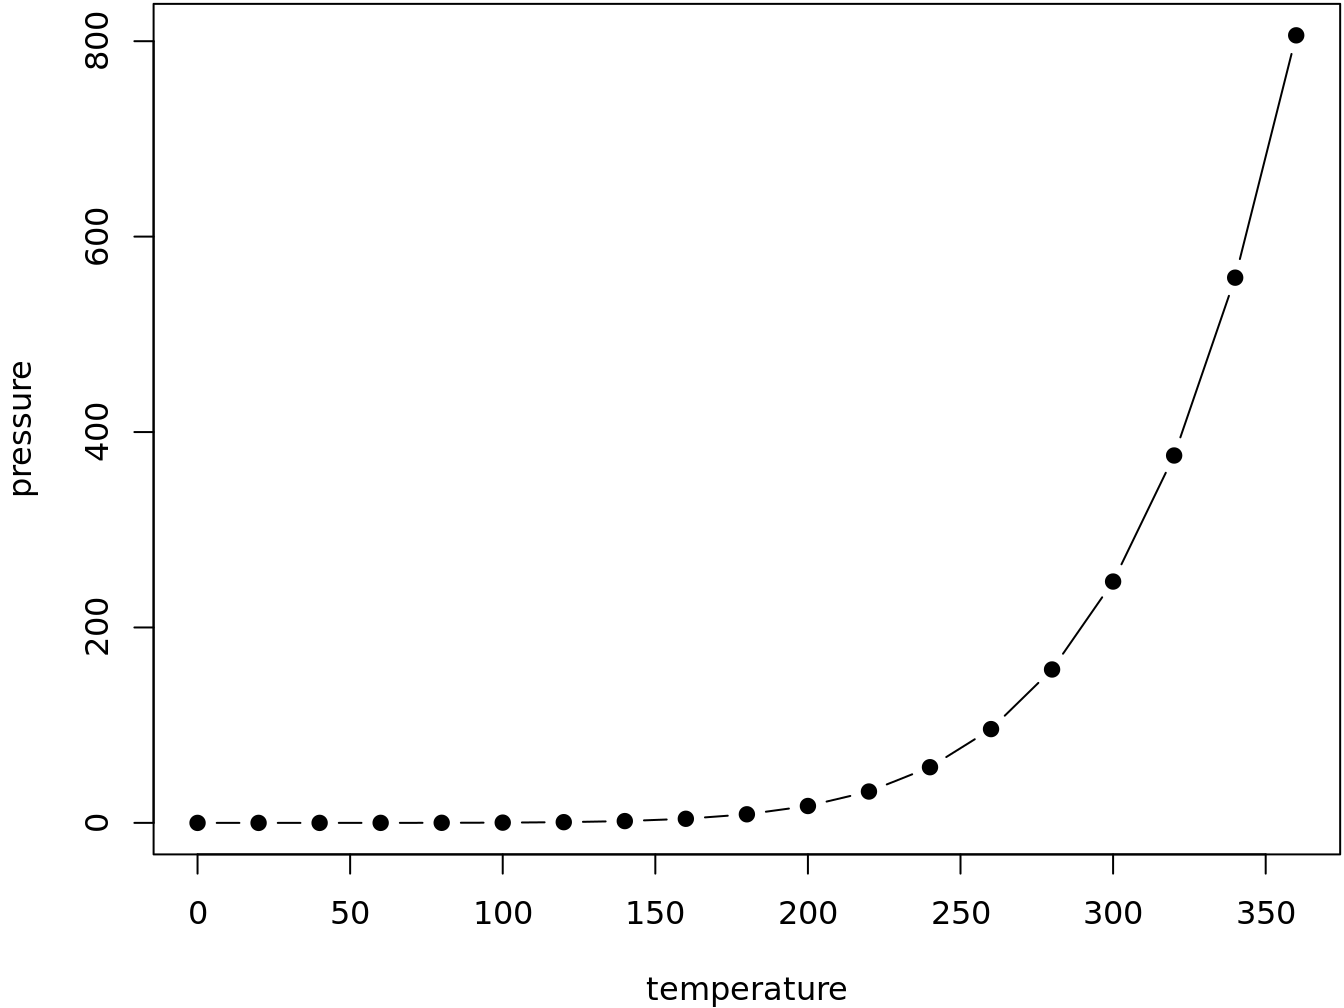
\includegraphics[width=0.8\linewidth]{synthetic_bookdown_files/figure-latex/nice-fig-1} 

}

\caption{Here is a nice figure!}\label{fig:nice-fig}
\end{figure}

Reference a figure by its code chunk label with the \texttt{fig:} prefix, e.g., see Figure \ref{fig:nice-fig}. Similarly, you can reference tables generated from \texttt{knitr::kable()}, e.g., see Table \ref{tab:nice-tab}.

\begin{Shaded}
\begin{Highlighting}[]
\NormalTok{knitr}\OperatorTok{::}\KeywordTok{kable}\NormalTok{(}
  \KeywordTok{head}\NormalTok{(iris, }\DecValTok{20}\NormalTok{), }\DataTypeTok{caption =} \StringTok{'Here is a nice table!'}\NormalTok{,}
  \DataTypeTok{booktabs =} \OtherTok{TRUE}
\NormalTok{)}
\end{Highlighting}
\end{Shaded}

\begin{table}

\caption{\label{tab:nice-tab}Here is a nice table!}
\centering
\begin{tabular}[t]{rrrrl}
\toprule
Sepal.Length & Sepal.Width & Petal.Length & Petal.Width & Species\\
\midrule
5.1 & 3.5 & 1.4 & 0.2 & setosa\\
4.9 & 3.0 & 1.4 & 0.2 & setosa\\
4.7 & 3.2 & 1.3 & 0.2 & setosa\\
4.6 & 3.1 & 1.5 & 0.2 & setosa\\
5.0 & 3.6 & 1.4 & 0.2 & setosa\\
\addlinespace
5.4 & 3.9 & 1.7 & 0.4 & setosa\\
4.6 & 3.4 & 1.4 & 0.3 & setosa\\
5.0 & 3.4 & 1.5 & 0.2 & setosa\\
4.4 & 2.9 & 1.4 & 0.2 & setosa\\
4.9 & 3.1 & 1.5 & 0.1 & setosa\\
\addlinespace
5.4 & 3.7 & 1.5 & 0.2 & setosa\\
4.8 & 3.4 & 1.6 & 0.2 & setosa\\
4.8 & 3.0 & 1.4 & 0.1 & setosa\\
4.3 & 3.0 & 1.1 & 0.1 & setosa\\
5.8 & 4.0 & 1.2 & 0.2 & setosa\\
\addlinespace
5.7 & 4.4 & 1.5 & 0.4 & setosa\\
5.4 & 3.9 & 1.3 & 0.4 & setosa\\
5.1 & 3.5 & 1.4 & 0.3 & setosa\\
5.7 & 3.8 & 1.7 & 0.3 & setosa\\
5.1 & 3.8 & 1.5 & 0.3 & setosa\\
\bottomrule
\end{tabular}
\end{table}

You can write citations, too. For example, we are using the \textbf{bookdown} package \citep{R-bookdown} in this sample book, which was built on top of R Markdown and \textbf{knitr} \citep{xie2015}.

WHat goes in here:

motivation
overview of steps
Prerequisites

\hypertarget{assumptions}{%
\section{Assumptions}\label{assumptions}}

It is assumed that the reader is familiar with the basic concepts and motivations around using DataSHIELD for federated analysis. More information about this can be found \href{https://isglobal-brge.github.io/resource_bookdown/datashield.html}{here}.

Knowledge of R. For harmonisation, knowledge of JavaScript and or MagmaScript is needed. For analysis, an understanding of DSLite.

(\textbf{TO DO add some more links to helpful stuff here})

\hypertarget{motivation}{%
\section{Motivation}\label{motivation}}

The benefits of the federated approach are that data can be harmonised and analysed without giving complete access to or transferring the data. A less desirable consequence of this approach is that it is more challenging for data experts to harmonise data to common standards, and for analysts to run their scripts, when the data are not tangibly in front of them. One could say that it is like trying to build a Lego model while wearing a blindfold.

With harmonisation, some groups have been through the process of transferring and centralising the data, but this negates one of the benefits of the federated approach. While it is only necessary for the harmonisation team to receive the data, a lot of bureaucracy is required. Others have mandated that each group harmonise their own data. The challenge with this approach is that there can be inconsistencies in the approach of different teams, and each team needs training and expertise in the harmonisation process.

Analysis via DataSHIELD has no such compromises and requires the analyst to make their own checks to validate that their analysis is progressing as planned. For example, to confirm that a subset into male and female groups has been successful, the analyst could ask for a summary of the original gender column and check the counts of male and female participants match the length of the subset dataframes. These extra steps are fine, but it can be more tricky to confirm the behaviour of more complex functions such as \texttt{ds.lexis} and \texttt{ds.reshape}.

\hypertarget{hypothesis-for-using-synthetic-data}{%
\section{Hypothesis for using synthetic data}\label{hypothesis-for-using-synthetic-data}}

R packages like \textbf{synthpop} \citep{synthpop} have been developed to generate realistic synthetic data that is not disclosive. A dsSynthpop package could be used to generate a synthetic data set on the client side by running the generation on the server side. Users can then perform harmonisation while working with full access to synthetic data on the client to confirm algorithms are working as expected. When the user is happy that the algorithms are working correctly, they can then be applied to the real data on the server side. The user therefore has the benefit of being able to see the data they are working with, but without the need to go through labourious data transfer processes. The same benefits are realised for an analysis user.

Other packages that provide synthetic data generation are \textbf{simstudy} and \textbf{gcipdr}. Simstudy requires the user to define the characteristics of variables and their relationships. However, access via DataSHIELD can help provide these summary statistics. There is also the benefit that the user then has precise control over the nature of the synthetic data generated. Likewise, gcipdr makes it easy for users to extract features such as mean, standard deviation and correlations via DataSHIELD, and use these to provide a more automated generation of the synthetic data.

\hypertarget{overview-of-steps}{%
\section{Overview of steps}\label{overview-of-steps}}

The hypothesis can be described by the following steps for harmonisation:

\begin{enumerate}
\def\labelenumi{\arabic{enumi}.}
\tightlist
\item
  The data custodian uploads the raw data to the server side and installs the server side pack \texttt{dsSynthetic}
\item
  The user install the package \texttt{dsSyntheticClient} on the client side
\item
  The user calls functions in the \texttt{dsSyntheticClient} package to generate a synthetic but non-disclosive data set which is returned to the client side.
\item
  With the synthetic data on the client side, the user can view the data and build harmonisation algorithms. They will be able to see the results of the algorithms for each row of data.
\item
  When the algorithms are complete, they can be implemented on Opal using the real data.
\end{enumerate}

And for analysis:

\begin{enumerate}
\def\labelenumi{\arabic{enumi}.}
\tightlist
\item
  Assuming steps \#1 and \#2 above are complete, the user calls functions in the \texttt{dsSyntheticClient} package to generate a synthetic but non-disclosive data set which is returned to the client side.
\item
  With the synthetic data on the client side, the user then starts a \texttt{DSLite} instance and places the synthetic data into it.
\item
  The user can then write their analysis using DataSHIELD commands against the DSLite instance. DSLite then allows the user to return any object on the server side. Therefore users can see the results of each step of their script for each row of data.
\item
  When the analysis script is complete, the user can run it against the real data on the server side.
\end{enumerate}

\hypertarget{prerequisites-1}{%
\section{Prerequisites}\label{prerequisites-1}}

Using DataSHIELD also requires some R packages to be installed on the client site. So far, the following R packages must be installed (in their development version):

\begin{Shaded}
\begin{Highlighting}[]
\KeywordTok{install.packages}\NormalTok{(}\StringTok{"DSOpal"}\NormalTok{, }\DataTypeTok{dependencies =} \OtherTok{TRUE}\NormalTok{)}
\KeywordTok{install.packages}\NormalTok{(}\StringTok{"dsBaseClient"}\NormalTok{, }\DataTypeTok{repos =} \KeywordTok{c}\NormalTok{(}\StringTok{"https://cloud.r-project.org"}\NormalTok{, }\StringTok{"https://cran.obiba.org"}\NormalTok{), }\DataTypeTok{dependencies =} \OtherTok{TRUE}\NormalTok{)}
\NormalTok{devtools}\OperatorTok{::}\KeywordTok{install_github}\NormalTok{(}\StringTok{"tombisho/dsSyntheticClient"}\NormalTok{, }\DataTypeTok{dependencies =} \OtherTok{TRUE}\NormalTok{)}
\KeywordTok{install.packages}\NormalTok{(}\StringTok{"simstudy"}\NormalTok{)}
\end{Highlighting}
\end{Shaded}

The package dependencies are then loaded as follows:

\begin{Shaded}
\begin{Highlighting}[]
\KeywordTok{library}\NormalTok{(DSOpal)}
\end{Highlighting}
\end{Shaded}

\begin{verbatim}
## Loading required package: opalr
\end{verbatim}

\begin{verbatim}
## Loading required package: httr
\end{verbatim}

\begin{verbatim}
## Loading required package: DSI
\end{verbatim}

\begin{verbatim}
## Loading required package: progress
\end{verbatim}

\begin{verbatim}
## Loading required package: R6
\end{verbatim}

\begin{Shaded}
\begin{Highlighting}[]
\KeywordTok{library}\NormalTok{(dsSyntheticClient)}
\end{Highlighting}
\end{Shaded}

\hypertarget{synthpop}{%
\chapter{Generating data using synthpop methods}\label{synthpop}}

In this chapter we will look at how to generate synthetic data on the server side using DataSHIELD functions, based on \textbf{synthpop} functionality.

First we need to build a login object for the server that holds the data:

\begin{Shaded}
\begin{Highlighting}[]
\NormalTok{builder <-}\StringTok{ }\NormalTok{DSI}\OperatorTok{::}\KeywordTok{newDSLoginBuilder}\NormalTok{()}
\CommentTok{# hide credentials}
\NormalTok{builder}\OperatorTok{$}\KeywordTok{append}\NormalTok{(}\DataTypeTok{server=}\StringTok{"server1"}\NormalTok{, }\DataTypeTok{url=}\StringTok{"https://opal-sandbox.mrc-epid.cam.ac.uk"}\NormalTok{,}
               \DataTypeTok{user=}\StringTok{"dsuser"}\NormalTok{, }\DataTypeTok{password=}\StringTok{"password"}\NormalTok{, }
               \DataTypeTok{table =} \StringTok{"DASIM.DASIM1"}\NormalTok{)}
\NormalTok{logindata <-}\StringTok{ }\NormalTok{builder}\OperatorTok{$}\KeywordTok{build}\NormalTok{()}
\end{Highlighting}
\end{Shaded}

And then we establish a connection to the server:

\begin{Shaded}
\begin{Highlighting}[]
\KeywordTok{library}\NormalTok{(DSOpal)}
\ControlFlowTok{if}\NormalTok{(}\KeywordTok{exists}\NormalTok{(}\StringTok{"connections"}\NormalTok{))\{}
  \KeywordTok{datashield.logout}\NormalTok{(}\DataTypeTok{conns =}\NormalTok{ connections)}
\NormalTok{\}}
\NormalTok{connections <-}\StringTok{ }\KeywordTok{datashield.login}\NormalTok{(}\DataTypeTok{logins=}\NormalTok{logindata, }\DataTypeTok{assign =} \OtherTok{TRUE}\NormalTok{)}
\end{Highlighting}
\end{Shaded}

\begin{verbatim}
## 
## Logging into the collaborating servers
\end{verbatim}

\begin{verbatim}
## 
##   No variables have been specified. 
##   All the variables in the table 
##   (the whole dataset) will be assigned to R!
\end{verbatim}

\begin{verbatim}
## 
## Assigning table data...
\end{verbatim}

The first option is to generate a synthetic dataset using an implementation of the \textbf{synthpop} package on the server side. \textbf{synthpop} requires some thought on the part of the user: if you have a data set with a large number of columns it may take a large amount of time to generate the synthetic data. Assuming we have a data set with a small number of columns (i.e.~around 10) we can simply execute the following command:

\begin{Shaded}
\begin{Highlighting}[]
\KeywordTok{library}\NormalTok{(dsSyntheticClient)}
\KeywordTok{library}\NormalTok{(dsBaseClient)}
\NormalTok{synth_data =}\StringTok{ }\KeywordTok{ds.syn}\NormalTok{(}\DataTypeTok{data =} \StringTok{"D"}\NormalTok{, }\DataTypeTok{method =} \StringTok{"cart"}\NormalTok{, }\DataTypeTok{m =} \DecValTok{1}\NormalTok{, }\DataTypeTok{seed =} \DecValTok{123}\NormalTok{)}\OperatorTok{$}\NormalTok{server1}\OperatorTok{$}\NormalTok{syn}
\end{Highlighting}
\end{Shaded}

We then have the synthetic data on the client side and can view and manipulate it as required:

\begin{Shaded}
\begin{Highlighting}[]
\KeywordTok{head}\NormalTok{(synth_data)}
\end{Highlighting}
\end{Shaded}

\begin{verbatim}
##       LAB_TSC  LAB_TRIG  LAB_HDL LAB_GLUC_FASTING PM_BMI_CONTINUOUS DIS_CVA
## 1009 4.320998 0.9221068 1.932509         4.588154          24.25248       0
## 1012 7.932947 3.4311492 1.231556         4.234590          37.27944       0
## 1013 6.465673 2.3991640 1.384120         4.385473          38.09126       0
## 1014 7.055100 1.1889880 1.935859         3.722485          23.25954       0
## 1015 5.247587 1.8073161 1.283847         5.615076          28.56968       0
## 1016 7.443416 3.0247684 1.652697         5.540567          30.72788       0
##      DIS_DIAB DIS_AMI GENDER PM_BMI_CATEGORICAL
## 1009        0       0      1                  1
## 1012        0       0      1                  3
## 1013        0       0      0                  3
## 1014        0       0      0                  1
## 1015        0       0      0                  2
## 1016        0       0      0                  3
\end{verbatim}

If you have a dataset with a larger number of columns, you could generate a synthetic dataset for a subset of the variables that you need to generate a particular harmonised variable. For example if we needed to generate a diabetes variable based on blood triglycerides, HDL and glucose we could just generate a dataset for those variables:

\begin{Shaded}
\begin{Highlighting}[]
\KeywordTok{ds.subset}\NormalTok{(}\DataTypeTok{x =} \StringTok{"D"}\NormalTok{, }\DataTypeTok{subset =} \StringTok{"D2"}\NormalTok{, }\DataTypeTok{cols =} \KeywordTok{c}\NormalTok{(}\StringTok{"LAB_HDL"}\NormalTok{, }\StringTok{"LAB_TRIG"}\NormalTok{, }\StringTok{"LAB_GLUC_FASTING"}\NormalTok{))}
\end{Highlighting}
\end{Shaded}

\begin{verbatim}
## Warning: 'ds.subset' is deprecated.
## Use 'ds.dataFrameSubset' instead.
## See help("Deprecated")
\end{verbatim}

\begin{Shaded}
\begin{Highlighting}[]
\NormalTok{synth_data_sub =}\StringTok{ }\KeywordTok{ds.syn}\NormalTok{(}\DataTypeTok{data =} \StringTok{"D2"}\NormalTok{, }\DataTypeTok{method =} \StringTok{"cart"}\NormalTok{, }\DataTypeTok{m =} \DecValTok{1}\NormalTok{, }\DataTypeTok{seed =} \DecValTok{123}\NormalTok{)}\OperatorTok{$}\NormalTok{server1}\OperatorTok{$}\NormalTok{syn}
\KeywordTok{head}\NormalTok{(synth_data_sub)}
\end{Highlighting}
\end{Shaded}

\begin{verbatim}
##        LAB_HDL   LAB_TRIG LAB_GLUC_FASTING
## 1009 1.7714508  0.7221808         5.638771
## 1012 0.9774569  1.5153916         6.209230
## 1013 0.9881049  3.1658461         5.350550
## 1014 2.0103355 -0.3515943         3.331889
## 1015 1.9042037 -0.2851747         4.988254
## 1016 1.2544094  1.2883607         3.967962
\end{verbatim}

Lastly we save our data for later chapters:

\begin{Shaded}
\begin{Highlighting}[]
\KeywordTok{write.csv}\NormalTok{(}\DataTypeTok{x =}\NormalTok{ synth_data, }\DataTypeTok{file =} \StringTok{"synth_data.csv"}\NormalTok{)}
\end{Highlighting}
\end{Shaded}

\hypertarget{methods}{%
\chapter{Methods}\label{methods}}

We describe our methods in this chapter.

\hypertarget{generating-data-using-simstudy-methods}{%
\chapter{Generating data using simstudy methods}\label{generating-data-using-simstudy-methods}}

In this chapter we will look at how to generate synthetic data on the client side using DataSHIELD functions to extract characteristics of the data set from the server side.

Again we need to build a login object for the server that holds the data:

\begin{Shaded}
\begin{Highlighting}[]
\NormalTok{builder <-}\StringTok{ }\NormalTok{DSI}\OperatorTok{::}\KeywordTok{newDSLoginBuilder}\NormalTok{()}
\CommentTok{# hide credentials}
\NormalTok{builder}\OperatorTok{$}\KeywordTok{append}\NormalTok{(}\DataTypeTok{server=}\StringTok{"server1"}\NormalTok{, }\DataTypeTok{url=}\StringTok{"https://opal-sandbox.mrc-epid.cam.ac.uk"}\NormalTok{,}
               \DataTypeTok{user=}\StringTok{"dsuser"}\NormalTok{, }\DataTypeTok{password=}\StringTok{"password"}\NormalTok{, }
               \DataTypeTok{table =} \StringTok{"DASIM.DASIM1"}\NormalTok{)}
\NormalTok{logindata <-}\StringTok{ }\NormalTok{builder}\OperatorTok{$}\KeywordTok{build}\NormalTok{()}
\end{Highlighting}
\end{Shaded}

And then we establish a connection to the server:

\begin{Shaded}
\begin{Highlighting}[]
\KeywordTok{library}\NormalTok{(DSOpal)}
\ControlFlowTok{if}\NormalTok{(}\KeywordTok{exists}\NormalTok{(}\StringTok{"connections"}\NormalTok{))\{}
  \KeywordTok{datashield.logout}\NormalTok{(}\DataTypeTok{conns =}\NormalTok{ connections)}
\NormalTok{\}}
\NormalTok{connections <-}\StringTok{ }\KeywordTok{datashield.login}\NormalTok{(}\DataTypeTok{logins=}\NormalTok{logindata, }\DataTypeTok{assign =} \OtherTok{TRUE}\NormalTok{)}
\end{Highlighting}
\end{Shaded}

\begin{verbatim}
## 
## Logging into the collaborating servers
\end{verbatim}

\begin{verbatim}
## 
##   No variables have been specified. 
##   All the variables in the table 
##   (the whole dataset) will be assigned to R!
\end{verbatim}

\begin{verbatim}
## 
## Assigning table data...
\end{verbatim}

This method builds on the fundamentals of the \textbf{simstudy} package. There is a good introduction to this package \href{https://kgoldfeld.github.io/simstudy/index.html}{here}.

First we load the library

\begin{Shaded}
\begin{Highlighting}[]
\KeywordTok{library}\NormalTok{(}\StringTok{"simstudy"}\NormalTok{)}
\KeywordTok{library}\NormalTok{(}\StringTok{"dsBaseClient"}\NormalTok{)}
\end{Highlighting}
\end{Shaded}

Then we can extract some parameters from the real data using DataSHIELD commands and use these to generate our synthetic data.

We will look at the binary variables first, and get the probabilities for 0/1:

\begin{Shaded}
\begin{Highlighting}[]
\NormalTok{factor_vars =}\StringTok{ }\KeywordTok{c}\NormalTok{(}\StringTok{"DIS_CVA"}\NormalTok{, }\StringTok{"DIS_DIAB"}\NormalTok{, }\StringTok{"DIS_AMI"}\NormalTok{ )}
\NormalTok{probs =}\StringTok{ }\KeywordTok{numeric}\NormalTok{()}
\ControlFlowTok{for}\NormalTok{(var }\ControlFlowTok{in}\NormalTok{ factor_vars)\{}
  \KeywordTok{ds.asNumeric}\NormalTok{(}\KeywordTok{paste0}\NormalTok{(}\StringTok{"D$"}\NormalTok{,var), }\DataTypeTok{newobj =} \KeywordTok{paste0}\NormalTok{(var,}\StringTok{"_num"}\NormalTok{), }\DataTypeTok{datasources =}\NormalTok{ connections)}
\NormalTok{  probs =}\StringTok{ }\KeywordTok{c}\NormalTok{(probs, }\KeywordTok{ds.mean}\NormalTok{(}\KeywordTok{paste0}\NormalTok{(var,}\StringTok{"_num"}\NormalTok{), }\DataTypeTok{datasources =}\NormalTok{ connections)}\OperatorTok{$}\NormalTok{Mean.by.Study[}\DecValTok{1}\NormalTok{])}
\NormalTok{\}}
\end{Highlighting}
\end{Shaded}

Now we use \textbf{simstudy} to generate the binary variables:

\begin{Shaded}
\begin{Highlighting}[]
\NormalTok{def <-}\StringTok{ }\KeywordTok{defData}\NormalTok{(}\DataTypeTok{varname =} \StringTok{"GENDER"}\NormalTok{, }\DataTypeTok{dist =} \StringTok{"binary"}\NormalTok{, }
               \DataTypeTok{formula =} \StringTok{"0.5"}\NormalTok{)}
\NormalTok{def <-}\StringTok{ }\KeywordTok{defData}\NormalTok{(def, }\DataTypeTok{varname =} \StringTok{"DIS_CVA"}\NormalTok{, }\DataTypeTok{dist =} \StringTok{"binary"}\NormalTok{, }
               \DataTypeTok{formula =}\NormalTok{ probs[}\DecValTok{1}\NormalTok{])}
\NormalTok{def <-}\StringTok{ }\KeywordTok{defData}\NormalTok{(def, }\DataTypeTok{varname =} \StringTok{"DIS_DIAB"}\NormalTok{, }\DataTypeTok{dist =} \StringTok{"binary"}\NormalTok{, }
               \DataTypeTok{formula =}\NormalTok{ probs[}\DecValTok{2}\NormalTok{])}
\NormalTok{def <-}\StringTok{ }\KeywordTok{defData}\NormalTok{(def, }\DataTypeTok{varname =} \StringTok{"DIS_AMI"}\NormalTok{, }\DataTypeTok{dist =} \StringTok{"binary"}\NormalTok{, }
               \DataTypeTok{formula =}\NormalTok{ probs[}\DecValTok{3}\NormalTok{])}
\NormalTok{synth_data_sim <-}\StringTok{ }\KeywordTok{genData}\NormalTok{(}\DecValTok{1000}\NormalTok{, def)}
\end{Highlighting}
\end{Shaded}

There are some variables that we expect to be normally distributed, so we will extract the mean and standard deviation:

\begin{Shaded}
\begin{Highlighting}[]
\NormalTok{columns =}\StringTok{ }\KeywordTok{c}\NormalTok{(}\StringTok{"LAB_TSC"}\NormalTok{, }\StringTok{"LAB_TRIG"}\NormalTok{, }\StringTok{"LAB_HDL"}\NormalTok{, }\StringTok{"LAB_GLUC_FASTING"}\NormalTok{, }\StringTok{"PM_BMI_CONTINUOUS"}\NormalTok{)}
\NormalTok{means =}\StringTok{ }\KeywordTok{numeric}\NormalTok{()}
\NormalTok{sds =}\StringTok{ }\KeywordTok{numeric}\NormalTok{()}
\ControlFlowTok{for}\NormalTok{ (var }\ControlFlowTok{in}\NormalTok{ columns)\{}
\NormalTok{  means =}\StringTok{ }\KeywordTok{c}\NormalTok{(means, }\KeywordTok{ds.mean}\NormalTok{(}\KeywordTok{paste0}\NormalTok{(}\StringTok{"D$"}\NormalTok{,var), }\DataTypeTok{datasources =}\NormalTok{ connections)}\OperatorTok{$}\NormalTok{Mean.by.Study[}\DecValTok{1}\NormalTok{])}
\NormalTok{  sds =}\StringTok{ }\KeywordTok{c}\NormalTok{(sds, }\KeywordTok{ds.var}\NormalTok{(}\KeywordTok{paste0}\NormalTok{(}\StringTok{"D$"}\NormalTok{,var), }\DataTypeTok{datasources =}\NormalTok{ connections)}\OperatorTok{$}\NormalTok{Variance.by.Study[}\DecValTok{1}\NormalTok{]}\OperatorTok{^}\FloatTok{0.5}\NormalTok{)}
\NormalTok{      \}}
\end{Highlighting}
\end{Shaded}

We can obtain the correlation matrix from DataSHIELD:

\begin{Shaded}
\begin{Highlighting}[]
\NormalTok{corrs =}\StringTok{ }\KeywordTok{ds.cor}\NormalTok{(}\DataTypeTok{x=}\StringTok{"D"}\NormalTok{, }\DataTypeTok{datasources =}\NormalTok{ connections)[[}\DecValTok{1}\NormalTok{]]}\OperatorTok{$}\StringTok{`}\DataTypeTok{Correlation Matrix}\StringTok{`}
\NormalTok{Dnames =}\StringTok{ }\KeywordTok{ds.colnames}\NormalTok{(}\StringTok{"D"}\NormalTok{)}\OperatorTok{$}\NormalTok{server1}
\KeywordTok{colnames}\NormalTok{(corrs) <-}\StringTok{ }\NormalTok{Dnames}
\KeywordTok{rownames}\NormalTok{(corrs) <-}\StringTok{ }\NormalTok{Dnames}
\end{Highlighting}
\end{Shaded}

And use the correlation matrix and the properties of the normally distributed data to generate simulated data for them, adding this to the binary data we already generated:

\begin{Shaded}
\begin{Highlighting}[]
\NormalTok{synth_data_sim <-}\StringTok{ }\KeywordTok{addCorData}\NormalTok{(synth_data_sim, }\DataTypeTok{idname =} \StringTok{"id"}\NormalTok{, }\DataTypeTok{mu =}\NormalTok{ means, }\DataTypeTok{sigma =}\NormalTok{ sds, }\DataTypeTok{corMatrix =}\NormalTok{ corrs[}\KeywordTok{c}\NormalTok{(}\DecValTok{1}\OperatorTok{:}\DecValTok{5}\NormalTok{), }\KeywordTok{c}\NormalTok{(}\DecValTok{1}\OperatorTok{:}\DecValTok{5}\NormalTok{)], }\DataTypeTok{cnames =}\NormalTok{ columns)}
\KeywordTok{head}\NormalTok{(synth_data_sim)}
\end{Highlighting}
\end{Shaded}

\begin{verbatim}
##    id GENDER DIS_CVA DIS_DIAB DIS_AMI  LAB_TSC  LAB_TRIG   LAB_HDL
## 1:  1      1       0        0       0 5.964282 3.4825556 0.6435067
## 2:  2      1       0        0       0 6.083158 1.2077771 1.6038941
## 3:  3      1       0        0       0 5.331941 2.3948606 1.8083096
## 4:  4      0       0        0       0 5.228991 2.4034744 1.6068916
## 5:  5      0       0        0       0 6.359223 0.6829469 1.5904361
## 6:  6      1       0        0       0 5.069500 2.5930527 2.0297472
##    LAB_GLUC_FASTING PM_BMI_CONTINUOUS
## 1:         4.944612          29.14046
## 2:         3.935429          29.98489
## 3:         4.513381          21.06302
## 4:         5.984858          25.79014
## 5:         4.356106          29.53963
## 6:         4.890059          28.85349
\end{verbatim}

\textbf{TO DO} the binary data and normal data are not linked through the correlation. I wonder how this could be done to improve the realism of the data.

\hypertarget{generating-data-using-gcipdr-methods}{%
\chapter{Generating data using gcipdr methods}\label{generating-data-using-gcipdr-methods}}

In this chapter we will look at how to generate synthetic data on the client side using DataSHIELD functions to extract characteristics of the data set from the server side.

The \textbf{gcipdr} package is an initial version and more details can be found \href{https://github.com/bonorico/gcipdr}{here}.

More prerequisites:

\begin{Shaded}
\begin{Highlighting}[]
\KeywordTok{library}\NormalTok{(devtools)}
\end{Highlighting}
\end{Shaded}

\begin{verbatim}
## Loading required package: usethis
\end{verbatim}

\begin{Shaded}
\begin{Highlighting}[]
\KeywordTok{install_github}\NormalTok{(}\StringTok{"bonorico/gcipdr"}\NormalTok{)}
\end{Highlighting}
\end{Shaded}

\begin{verbatim}
## Skipping install of 'gcipdr' from a github remote, the SHA1 (59fc74f6) has not changed since last install.
##   Use `force = TRUE` to force installation
\end{verbatim}

\begin{Shaded}
\begin{Highlighting}[]
\NormalTok{url <-}\StringTok{ "https://cran.r-project.org/src/contrib/Archive/JohnsonDistribution/JohnsonDistribution_0.24.tar.gz"}
\NormalTok{pkgFile <-}\StringTok{ "JohnsonDistribution_0.24.tar.gz"}
\KeywordTok{download.file}\NormalTok{(}\DataTypeTok{url =}\NormalTok{ url, }\DataTypeTok{destfile =}\NormalTok{ pkgFile)}

\KeywordTok{install.packages}\NormalTok{(}\DataTypeTok{pkgs=}\NormalTok{pkgFile, }\DataTypeTok{type=}\StringTok{"source"}\NormalTok{, }\DataTypeTok{repos=}\OtherTok{NULL}\NormalTok{)}
\end{Highlighting}
\end{Shaded}

\begin{verbatim}
## Installing package into '/home/vagrant/R/x86_64-pc-linux-gnu-library/4.0'
## (as 'lib' is unspecified)
\end{verbatim}

\begin{Shaded}
\begin{Highlighting}[]
\KeywordTok{unlink}\NormalTok{(pkgFile)}
\end{Highlighting}
\end{Shaded}

Again we need to build a login object for the server that holds the data:

\begin{Shaded}
\begin{Highlighting}[]
\NormalTok{builder <-}\StringTok{ }\NormalTok{DSI}\OperatorTok{::}\KeywordTok{newDSLoginBuilder}\NormalTok{()}
\CommentTok{# hide credentials}
\NormalTok{builder}\OperatorTok{$}\KeywordTok{append}\NormalTok{(}\DataTypeTok{server=}\StringTok{"server1"}\NormalTok{, }\DataTypeTok{url=}\StringTok{"https://opal-sandbox.mrc-epid.cam.ac.uk"}\NormalTok{,}
               \DataTypeTok{user=}\StringTok{"dsuser"}\NormalTok{, }\DataTypeTok{password=}\StringTok{"password"}\NormalTok{, }
               \DataTypeTok{table =} \StringTok{"DASIM.DASIM1"}\NormalTok{)}
\NormalTok{logindata <-}\StringTok{ }\NormalTok{builder}\OperatorTok{$}\KeywordTok{build}\NormalTok{()}
\end{Highlighting}
\end{Shaded}

And then we establish a connection to the server:

\begin{Shaded}
\begin{Highlighting}[]
\KeywordTok{library}\NormalTok{(DSOpal)}
\ControlFlowTok{if}\NormalTok{(}\KeywordTok{exists}\NormalTok{(}\StringTok{"connections"}\NormalTok{))\{}
  \KeywordTok{datashield.logout}\NormalTok{(}\DataTypeTok{conns =}\NormalTok{ connections)}
\NormalTok{\}}
\NormalTok{connections <-}\StringTok{ }\KeywordTok{datashield.login}\NormalTok{(}\DataTypeTok{logins=}\NormalTok{logindata, }\DataTypeTok{assign =} \OtherTok{TRUE}\NormalTok{)}
\end{Highlighting}
\end{Shaded}

\begin{verbatim}
## 
## Logging into the collaborating servers
\end{verbatim}

\begin{verbatim}
## 
##   No variables have been specified. 
##   All the variables in the table 
##   (the whole dataset) will be assigned to R!
\end{verbatim}

\begin{verbatim}
## 
## Assigning table data...
\end{verbatim}

\hypertarget{harmonisation-with-synthetic-data}{%
\chapter{Harmonisation with synthetic data}\label{harmonisation-with-synthetic-data}}

In this section we describe how to harmonise synthetic data on the client side. This assumes that you have used one of the previous methods to generate your synthetic data set.

Recall that we are aiming to use synthetic data on the client side to design harmonisation algorithms, and then implement these on Opal on the server side using the real data. This removes the need for the user to have full access to the data. Harmonisation algorithms can be implemented in Opal using MagmaScript (JavaScript) without having full access to the data. The idea is that writing JavaScript on the client side, having full access to the synthetic data, is easier than writing the code on the server side with only access to summaries.

In detail, the steps proposed are:

\begin{enumerate}
\def\labelenumi{\arabic{enumi}.}
\tightlist
\item
  Start a JavaScript session on the client side
\item
  Load the synthetic data into the session
\item
  Write and test JavaScript code in the session against the synthetic data
\item
  When happy, copy the code into Opal to generate the harmonised data
\end{enumerate}

\hypertarget{getting-set-up}{%
\section{Getting set up}\label{getting-set-up}}

First some system level packages may need to be installed: On Debian / Ubuntu install either \texttt{libv8-dev} or \texttt{libnode-dev}, on Fedora use \texttt{v8-devel}.

\begin{Shaded}
\begin{Highlighting}[]
\KeywordTok{install.packages}\NormalTok{(}\StringTok{"V8"}\NormalTok{)}
\end{Highlighting}
\end{Shaded}

\begin{verbatim}
## Installing package into '/home/vagrant/R/x86_64-pc-linux-gnu-library/4.0'
## (as 'lib' is unspecified)
\end{verbatim}

\begin{Shaded}
\begin{Highlighting}[]
\KeywordTok{library}\NormalTok{(}\StringTok{"V8"}\NormalTok{)}
\end{Highlighting}
\end{Shaded}

\begin{verbatim}
## Using V8 engine 6.8.275.32-node.12
\end{verbatim}

\hypertarget{do-the-work}{%
\section{Do the work}\label{do-the-work}}

Now we can start a JavaScript session and load the additional MagmaScript functionality:

\begin{Shaded}
\begin{Highlighting}[]
\NormalTok{ct2 =}\StringTok{ }\KeywordTok{v8}\NormalTok{()}
\NormalTok{ct2}\OperatorTok{$}\KeywordTok{source}\NormalTok{(}\StringTok{"https://raw.githubusercontent.com/tombisho/dsSyntheticClient/main/MagmaScript.min.js"}\NormalTok{)}
\end{Highlighting}
\end{Shaded}

\begin{verbatim}
## [1] "true"
\end{verbatim}

\begin{Shaded}
\begin{Highlighting}[]
\NormalTok{synth_data =}\StringTok{ }\KeywordTok{read.csv}\NormalTok{(}\DataTypeTok{file =} \StringTok{"synth_data.csv"}\NormalTok{)}
\NormalTok{ct2}\OperatorTok{$}\KeywordTok{assign}\NormalTok{(}\StringTok{"synth_data"}\NormalTok{, synth_data)}
\end{Highlighting}
\end{Shaded}

We then go into the console, grab a row of data and write some JavaScript:

\begin{Shaded}
\begin{Highlighting}[]
\NormalTok{ct2}\OperatorTok{$}\KeywordTok{console}\NormalTok{()}
\end{Highlighting}
\end{Shaded}

\begin{Shaded}
\begin{Highlighting}[]

\KeywordTok{var}\NormalTok{ $ }\OperatorTok{=} \VariableTok{MagmaScript}\NormalTok{.}\VariableTok{MagmaScript}\NormalTok{.}\VariableTok{$}\NormalTok{.}\AttributeTok{bind}\NormalTok{(als_syn[}\DecValTok{0}\NormalTok{])}\OperatorTok{;}

\ControlFlowTok{if}\NormalTok{ (}\AttributeTok{$}\NormalTok{(}\StringTok{'y3age'}\NormalTok{).}\AttributeTok{value}\NormalTok{() }\OperatorTok{>} \DecValTok{25}\NormalTok{ )}\OperatorTok{\{}
\NormalTok{  out }\OperatorTok{=} \DecValTok{1}
\OperatorTok{\}} \ControlFlowTok{else} \OperatorTok{\{}
\NormalTok{  out }\OperatorTok{=} \DecValTok{0}
\OperatorTok{\}}
\end{Highlighting}
\end{Shaded}

Now we test our code against the whole dataset:

\begin{Shaded}
\begin{Highlighting}[]

\NormalTok{myScript }\OperatorTok{=} \VerbatimStringTok{`}
\VerbatimStringTok{if ($('y3age').value() > 25 )\{}
\VerbatimStringTok{  out = 1}
\VerbatimStringTok{\} else \{}
\VerbatimStringTok{  out = 0}
\VerbatimStringTok{\}}
\VerbatimStringTok{`}

\KeywordTok{var}\NormalTok{ my_out }\OperatorTok{=}\NormalTok{ []}\OperatorTok{;}

\ControlFlowTok{for}\NormalTok{ (j }\OperatorTok{=} \DecValTok{0}\OperatorTok{;}\NormalTok{ j }\OperatorTok{<} \VariableTok{als_syn}\NormalTok{.}\AttributeTok{length}\OperatorTok{;}\NormalTok{ j}\OperatorTok{++}\NormalTok{)}\OperatorTok{\{}
  \VariableTok{my_out}\NormalTok{.}\AttributeTok{push}\NormalTok{(}\VariableTok{MagmaScript}\NormalTok{.}\AttributeTok{evaluator}\NormalTok{(myScript}\OperatorTok{,}\NormalTok{ als_syn[j]))}
\OperatorTok{\}}
\NormalTok{exit}
\end{Highlighting}
\end{Shaded}

And pull the results into R for inspection:

\begin{Shaded}
\begin{Highlighting}[]
\NormalTok{my_out =}\StringTok{ }\NormalTok{ct2}\OperatorTok{$}\KeywordTok{get}\NormalTok{(}\StringTok{"my_out"}\NormalTok{)}

\NormalTok{synth_data_harm =}\StringTok{ }\NormalTok{synth_data}
\NormalTok{synth_data_harm}\OperatorTok{$}\NormalTok{my_var =}\StringTok{ }\NormalTok{my_out}
\end{Highlighting}
\end{Shaded}

If we are happy with the code, we can paste it directly into the Opal \emph{script} interface so that it can be executed on the real data.

\hypertarget{analysis-with-synthetic-data}{%
\chapter{Analysis with synthetic data}\label{analysis-with-synthetic-data}}

In this section we describe how we can use a copy of the synthetic data to help users write DataSHIELD analysis code. Again we will make use of an existing dataset (** TO DO would be better to run this on some harmonised data)

Recall that the objective here is to use a synthetic copy of already harmonised real data that is then made available to the analyst on the client side. This synthetic data set can be loaded into \textbf{DSLite}, a special client side implementation of server side DataSHIELD used for development purposes: the user can have full access to the data. This is acceptable in this situation as the data are synthetic. Therefore the user has the chance to write DataSHIELD code but see the complete results of each step. This makes it easier to develop the code.

\hypertarget{getting-set-up-1}{%
\section{Getting set up}\label{getting-set-up-1}}

We require \texttt{DSLite} and \texttt{dsBase} to be installed:

\begin{Shaded}
\begin{Highlighting}[]
\KeywordTok{install.packages}\NormalTok{(}\KeywordTok{c}\NormalTok{(}\StringTok{"resourcer"}\NormalTok{, }\StringTok{"DSLite"}\NormalTok{), }\DataTypeTok{dependencies =} \OtherTok{TRUE}\NormalTok{)}
\end{Highlighting}
\end{Shaded}

\begin{verbatim}
## Installing packages into '/home/vagrant/R/x86_64-pc-linux-gnu-library/4.0'
## (as 'lib' is unspecified)
\end{verbatim}

\begin{verbatim}
## also installing the dependencies 'ssh', 'mongolite', 'RMariaDB', 'RPostgres'
\end{verbatim}

\begin{verbatim}
## Warning in install.packages(c("resourcer", "DSLite"), dependencies = TRUE):
## installation of package 'ssh' had non-zero exit status
\end{verbatim}

\begin{verbatim}
## Warning in install.packages(c("resourcer", "DSLite"), dependencies = TRUE):
## installation of package 'mongolite' had non-zero exit status
\end{verbatim}

\begin{verbatim}
## Warning in install.packages(c("resourcer", "DSLite"), dependencies = TRUE):
## installation of package 'RMariaDB' had non-zero exit status
\end{verbatim}

\begin{verbatim}
## Warning in install.packages(c("resourcer", "DSLite"), dependencies = TRUE):
## installation of package 'RPostgres' had non-zero exit status
\end{verbatim}

\begin{Shaded}
\begin{Highlighting}[]
\KeywordTok{install.packages}\NormalTok{(}\StringTok{"dsBase"}\NormalTok{, }\DataTypeTok{repos =} \KeywordTok{c}\NormalTok{(}\StringTok{"https://cloud.r-project.org"}\NormalTok{, }\StringTok{"https://cran.obiba.org"}\NormalTok{), }\DataTypeTok{dependencies =} \OtherTok{TRUE}\NormalTok{)}
\end{Highlighting}
\end{Shaded}

\begin{verbatim}
## Installing package into '/home/vagrant/R/x86_64-pc-linux-gnu-library/4.0'
## (as 'lib' is unspecified)
\end{verbatim}

Let us assume that the \emph{DASIM1} dataset has previously been harmonised and is held on a server. We do not have access to the full dataset but want to do some analysis on it. Using the method described above, the first thing to do is generate a synthetic version that we can fully access. To do this we will use the same steps that were shown in \citet{ref}(synthpop)

\hypertarget{create-synthetic-dataset}{%
\section{Create synthetic dataset}\label{create-synthetic-dataset}}

We build our log in object

\begin{Shaded}
\begin{Highlighting}[]
\NormalTok{builder <-}\StringTok{ }\NormalTok{DSI}\OperatorTok{::}\KeywordTok{newDSLoginBuilder}\NormalTok{()}
\NormalTok{builder}\OperatorTok{$}\KeywordTok{append}\NormalTok{(}\DataTypeTok{server=}\StringTok{"server1"}\NormalTok{, }\DataTypeTok{url=}\StringTok{"https://opal-sandbox.mrc-epid.cam.ac.uk"}\NormalTok{,}
               \DataTypeTok{user=}\StringTok{"dsuser"}\NormalTok{, }\DataTypeTok{password=}\StringTok{"password"}\NormalTok{, }
               \DataTypeTok{table =} \StringTok{"DASIM.DASIM1"}\NormalTok{)}
\NormalTok{logindata <-}\StringTok{ }\NormalTok{builder}\OperatorTok{$}\KeywordTok{build}\NormalTok{()}
\end{Highlighting}
\end{Shaded}

Then perform the log in to ther server:

\begin{Shaded}
\begin{Highlighting}[]
\KeywordTok{library}\NormalTok{(DSOpal)}
\ControlFlowTok{if}\NormalTok{(}\KeywordTok{exists}\NormalTok{(}\StringTok{"connections"}\NormalTok{))\{}
  \KeywordTok{datashield.logout}\NormalTok{(}\DataTypeTok{conns =}\NormalTok{ connections)}
\NormalTok{\}}
\NormalTok{connections <-}\StringTok{ }\KeywordTok{datashield.login}\NormalTok{(}\DataTypeTok{logins=}\NormalTok{logindata, }\DataTypeTok{assign =} \OtherTok{TRUE}\NormalTok{)}
\end{Highlighting}
\end{Shaded}

\begin{verbatim}
## 
## Logging into the collaborating servers
\end{verbatim}

\begin{verbatim}
## 
##   No variables have been specified. 
##   All the variables in the table 
##   (the whole dataset) will be assigned to R!
\end{verbatim}

\begin{verbatim}
## 
## Assigning table data...
\end{verbatim}

The \emph{DASIM1} dataset is relatively small (i.e.~around 10 columns). This is probably also true of many harmonised data sets.
Therefore we can just create a synthetic version of it:

\begin{Shaded}
\begin{Highlighting}[]
\KeywordTok{library}\NormalTok{(dsSyntheticClient)}
\NormalTok{synth_data =}\StringTok{ }\KeywordTok{ds.syn}\NormalTok{(}\DataTypeTok{data =} \StringTok{"D"}\NormalTok{, }\DataTypeTok{method =} \StringTok{"cart"}\NormalTok{, }\DataTypeTok{m =} \DecValTok{1}\NormalTok{, }\DataTypeTok{seed =} \DecValTok{123}\NormalTok{)}
\NormalTok{DASIM =}\StringTok{ }\NormalTok{synth_data}\OperatorTok{$}\NormalTok{server1}\OperatorTok{$}\NormalTok{syn}
\end{Highlighting}
\end{Shaded}

\hypertarget{start-dslite-local-instance}{%
\section{Start DSLite local instance}\label{start-dslite-local-instance}}

\begin{Shaded}
\begin{Highlighting}[]
\KeywordTok{library}\NormalTok{(DSLite)}
\KeywordTok{library}\NormalTok{(dsBaseClient)}
\NormalTok{dslite.server <-}\StringTok{ }\KeywordTok{newDSLiteServer}\NormalTok{(}\DataTypeTok{tables=}\KeywordTok{list}\NormalTok{(}\DataTypeTok{DASIM=}\NormalTok{DASIM))}
\NormalTok{dslite.server}\OperatorTok{$}\KeywordTok{config}\NormalTok{(}\KeywordTok{defaultDSConfiguration}\NormalTok{(}\DataTypeTok{include=}\KeywordTok{c}\NormalTok{(}\StringTok{"dsBase"}\NormalTok{, }\StringTok{"dsSynthetic"}\NormalTok{)))}

\NormalTok{builder <-}\StringTok{ }\NormalTok{DSI}\OperatorTok{::}\KeywordTok{newDSLoginBuilder}\NormalTok{()}
\NormalTok{builder}\OperatorTok{$}\KeywordTok{append}\NormalTok{(}\DataTypeTok{server=}\StringTok{"server1"}\NormalTok{, }\DataTypeTok{url=}\StringTok{"dslite.server"}\NormalTok{, }\DataTypeTok{table =} \StringTok{"DASIM"}\NormalTok{, }\DataTypeTok{driver =} \StringTok{"DSLiteDriver"}\NormalTok{)}
\NormalTok{logindata <-}\StringTok{ }\NormalTok{builder}\OperatorTok{$}\KeywordTok{build}\NormalTok{()}

\ControlFlowTok{if}\NormalTok{(}\KeywordTok{exists}\NormalTok{(}\StringTok{"connections"}\NormalTok{))\{}
  \KeywordTok{datashield.logout}\NormalTok{(}\DataTypeTok{conns =}\NormalTok{ connections)}
\NormalTok{\}}
\NormalTok{connections <-}\StringTok{ }\KeywordTok{datashield.login}\NormalTok{(}\DataTypeTok{logins=}\NormalTok{logindata, }\DataTypeTok{assign =} \OtherTok{TRUE}\NormalTok{)}
\end{Highlighting}
\end{Shaded}

\begin{verbatim}
## 
## Logging into the collaborating servers
\end{verbatim}

\begin{verbatim}
## 
##   No variables have been specified. 
##   All the variables in the table 
##   (the whole dataset) will be assigned to R!
\end{verbatim}

\begin{verbatim}
## 
## Assigning table data...
\end{verbatim}

We can now check for ourselves that our \emph{DASIM} data is in the DSLite server:

\begin{Shaded}
\begin{Highlighting}[]
\KeywordTok{ds.summary}\NormalTok{(}\StringTok{'D'}\NormalTok{)}
\end{Highlighting}
\end{Shaded}

\begin{verbatim}
## $server1
## $server1$class
## [1] "data.frame"
## 
## $server1$`number of rows`
## [1] 10000
## 
## $server1$`number of columns`
## [1] 10
## 
## $server1$`variables held`
##  [1] "LAB_TSC"            "LAB_TRIG"           "LAB_HDL"           
##  [4] "LAB_GLUC_FASTING"   "PM_BMI_CONTINUOUS"  "DIS_CVA"           
##  [7] "DIS_DIAB"           "DIS_AMI"            "GENDER"            
## [10] "PM_BMI_CATEGORICAL"
\end{verbatim}

Now suppose we want to subset the \emph{DASIM} data into men and women. We can use the \texttt{ds.subset} function:

\begin{Shaded}
\begin{Highlighting}[]
\KeywordTok{ds.subset}\NormalTok{(}\DataTypeTok{x=}\StringTok{"D"}\NormalTok{, }\DataTypeTok{subset =} \StringTok{"women"}\NormalTok{, }\DataTypeTok{logicalOperator =} \StringTok{"=="}\NormalTok{, }\DataTypeTok{threshold =} \DecValTok{1}\NormalTok{)}
\end{Highlighting}
\end{Shaded}

\begin{verbatim}
## Warning: 'ds.subset' is deprecated.
## Use 'ds.dataFrameSubset' instead.
## See help("Deprecated")
\end{verbatim}

With DSLite we have the chance to look at actually what happened in detail:

\begin{Shaded}
\begin{Highlighting}[]
\NormalTok{women =}\StringTok{ }\KeywordTok{getDSLiteData}\NormalTok{(}\DataTypeTok{conns =}\NormalTok{ connections, }\DataTypeTok{symbol =} \StringTok{"women"}\NormalTok{)}\OperatorTok{$}\NormalTok{server1}
\KeywordTok{head}\NormalTok{(women)}
\end{Highlighting}
\end{Shaded}

\begin{verbatim}
##       LAB_TSC  LAB_TRIG  LAB_HDL LAB_GLUC_FASTING PM_BMI_CONTINUOUS DIS_CVA
## 1009 4.320998 0.9221068 1.932509         4.588154          24.25248       0
## 1012 7.932947 3.4311492 1.231556         4.234590          37.27944       0
## 1013 6.465673 2.3991640 1.384120         4.385473          38.09126       0
## 1014 7.055100 1.1889880 1.935859         3.722485          23.25954       0
## 1015 5.247587 1.8073161 1.283847         5.615076          28.56968       0
## 1016 7.443416 3.0247684 1.652697         5.540567          30.72788       0
##      DIS_DIAB DIS_AMI GENDER PM_BMI_CATEGORICAL
## 1009        0       0      1                  1
## 1012        0       0      1                  3
## 1013        0       0      0                  3
## 1014        0       0      0                  1
## 1015        0       0      0                  2
## 1016        0       0      0                  3
\end{verbatim}

As you can see we made an error in our code but didn't get a warning. Let's make a correction and try again:

\begin{Shaded}
\begin{Highlighting}[]
\KeywordTok{ds.subset}\NormalTok{(}\DataTypeTok{x=}\StringTok{"D"}\NormalTok{, }\DataTypeTok{subset =} \StringTok{"women"}\NormalTok{, }\DataTypeTok{logicalOperator =} \StringTok{"GENDER=="}\NormalTok{, }\DataTypeTok{threshold =} \DecValTok{1}\NormalTok{)}
\end{Highlighting}
\end{Shaded}

\begin{verbatim}
## Warning: 'ds.subset' is deprecated.
## Use 'ds.dataFrameSubset' instead.
## See help("Deprecated")
\end{verbatim}

\begin{Shaded}
\begin{Highlighting}[]
\CommentTok{# get the data again}
\NormalTok{women =}\StringTok{ }\KeywordTok{getDSLiteData}\NormalTok{(}\DataTypeTok{conns =}\NormalTok{ connections, }\DataTypeTok{symbol =} \StringTok{"women"}\NormalTok{)}\OperatorTok{$}\NormalTok{server1}
\KeywordTok{head}\NormalTok{(women)}
\end{Highlighting}
\end{Shaded}

\begin{verbatim}
##       LAB_TSC  LAB_TRIG  LAB_HDL LAB_GLUC_FASTING PM_BMI_CONTINUOUS DIS_CVA
## 1009 4.320998 0.9221068 1.932509         4.588154          24.25248       0
## 1012 7.932947 3.4311492 1.231556         4.234590          37.27944       0
## 1022 4.530228 2.7351977 1.129350         5.454553          29.99532       0
## 1025 5.026717 1.3289150 1.312407         6.304016          31.75667       0
## 1026 4.901544 2.3027582 1.569712         4.529539          24.64352       0
## 1030 5.428203 0.2307445 1.865315         4.039755          34.83133       0
##      DIS_DIAB DIS_AMI GENDER PM_BMI_CATEGORICAL
## 1009        0       0      1                  1
## 1012        0       0      1                  3
## 1022        0       0      1                  2
## 1025        0       0      1                  3
## 1026        0       0      1                  1
## 1030        0       0      1                  3
\end{verbatim}

This now looks much better.

We can also compare results obtained via DataSHIELD with results on the actual data:

\begin{Shaded}
\begin{Highlighting}[]
\NormalTok{from_server =}\StringTok{ }\KeywordTok{ds.glm}\NormalTok{(}\DataTypeTok{formula =} \StringTok{"DIS_DIAB~PM_BMI_CONTINUOUS+LAB_TSC+LAB_HDL"}\NormalTok{, }\DataTypeTok{data =} \StringTok{"women"}\NormalTok{, }\DataTypeTok{family =} \StringTok{"binomial"}\NormalTok{)}
\end{Highlighting}
\end{Shaded}

\begin{verbatim}
## Warning: glm.fit: algorithm did not converge
\end{verbatim}

\begin{verbatim}
## Iteration 1...
\end{verbatim}

\begin{verbatim}
## Warning: glm.fit: algorithm did not converge
\end{verbatim}

\begin{verbatim}
## CURRENT DEVIANCE:      6920.38145071049
\end{verbatim}

\begin{verbatim}
## Iteration 2...
\end{verbatim}

\begin{verbatim}
## Warning: glm.fit: algorithm did not converge
\end{verbatim}

\begin{verbatim}
## CURRENT DEVIANCE:      1644.898633909
\end{verbatim}

\begin{verbatim}
## Iteration 3...
\end{verbatim}

\begin{verbatim}
## Warning: glm.fit: algorithm did not converge
\end{verbatim}

\begin{verbatim}
## CURRENT DEVIANCE:      969.852946084612
\end{verbatim}

\begin{verbatim}
## Iteration 4...
\end{verbatim}

\begin{verbatim}
## Warning: glm.fit: algorithm did not converge
\end{verbatim}

\begin{verbatim}
## CURRENT DEVIANCE:      817.043471506761
\end{verbatim}

\begin{verbatim}
## Iteration 5...
\end{verbatim}

\begin{verbatim}
## Warning: glm.fit: algorithm did not converge
\end{verbatim}

\begin{verbatim}
## CURRENT DEVIANCE:      793.793345220942
\end{verbatim}

\begin{verbatim}
## Iteration 6...
\end{verbatim}

\begin{verbatim}
## Warning: glm.fit: algorithm did not converge
\end{verbatim}

\begin{verbatim}
## CURRENT DEVIANCE:      792.418496420342
\end{verbatim}

\begin{verbatim}
## Iteration 7...
\end{verbatim}

\begin{verbatim}
## Warning: glm.fit: algorithm did not converge
\end{verbatim}

\begin{verbatim}
## CURRENT DEVIANCE:      792.40865932329
\end{verbatim}

\begin{verbatim}
## Iteration 8...
\end{verbatim}

\begin{verbatim}
## Warning: glm.fit: algorithm did not converge
\end{verbatim}

\begin{verbatim}
## CURRENT DEVIANCE:      792.408658693972
\end{verbatim}

\begin{verbatim}
## SUMMARY OF MODEL STATE after iteration 8
\end{verbatim}

\begin{verbatim}
## Current deviance 792.408658693972 on 4988 degrees of freedom
\end{verbatim}

\begin{verbatim}
## Convergence criterion TRUE (7.94082767858234e-10)
\end{verbatim}

\begin{verbatim}
## 
## beta: -4.37857656701888 0.0557933313333051 -0.0910864934167108 -0.515226753189616
\end{verbatim}

\begin{verbatim}
## 
## Information matrix overall:
\end{verbatim}

\begin{verbatim}
##                   (Intercept) PM_BMI_CONTINUOUS    LAB_TSC   LAB_HDL
## (Intercept)          76.59994          2204.650   434.9845  116.4032
## PM_BMI_CONTINUOUS  2204.65020         65152.696 12583.5568 3304.8417
## LAB_TSC             434.98451         12583.557  2556.5488  664.2433
## LAB_HDL             116.40315          3304.842   664.2433  187.2085
\end{verbatim}

\begin{verbatim}
## 
## Score vector overall:
\end{verbatim}

\begin{verbatim}
##                            [,1]
## (Intercept)       -3.069541e-07
## PM_BMI_CONTINUOUS -7.524081e-06
## LAB_TSC           -1.779797e-06
## LAB_HDL           -5.576668e-07
\end{verbatim}

\begin{verbatim}
## 
## Current deviance: 792.408658693972
\end{verbatim}

\begin{Shaded}
\begin{Highlighting}[]
\NormalTok{from_local =}\StringTok{ }\KeywordTok{glm}\NormalTok{(}\DataTypeTok{formula =} \StringTok{"DIS_DIAB~PM_BMI_CONTINUOUS+LAB_TSC+LAB_HDL"}\NormalTok{, }\DataTypeTok{data =}\NormalTok{ women, }\DataTypeTok{family =} \StringTok{"binomial"}\NormalTok{)}

\NormalTok{from_server}\OperatorTok{$}\NormalTok{coefficients}
\end{Highlighting}
\end{Shaded}

\begin{verbatim}
##                      Estimate Std. Error    z-value      p-value low0.95CI.LP
## (Intercept)       -4.37857657 1.10156871 -3.9748556 7.042197e-05 -6.537611563
## PM_BMI_CONTINUOUS  0.05579333 0.02645985  2.1086038 3.497879e-02  0.003932988
## LAB_TSC           -0.09108649 0.11089084 -0.8214068 4.114146e-01 -0.308428551
## LAB_HDL           -0.51522675 0.33679076 -1.5298126 1.260631e-01 -1.175324504
##                   high0.95CI.LP       P_OR low0.95CI.P_OR high0.95CI.P_OR
## (Intercept)          -2.2195416 0.01238782    0.001445849      0.09800932
## PM_BMI_CONTINUOUS     0.1076537 1.05737913    1.003940732      1.11366199
## LAB_TSC               0.1262556 0.91293874    0.734600437      1.13457209
## LAB_HDL               0.1448710 0.59736512    0.308718783      1.15589045
\end{verbatim}

\begin{Shaded}
\begin{Highlighting}[]
\NormalTok{from_local}\OperatorTok{$}\NormalTok{coefficients}
\end{Highlighting}
\end{Shaded}

\begin{verbatim}
##       (Intercept) PM_BMI_CONTINUOUS           LAB_TSC           LAB_HDL 
##       -4.37857657        0.05579333       -0.09108649       -0.51522675
\end{verbatim}

\textbf{TO DO make a more realistic example for example with ds.lexis or ds.reshape where it is much harder to know what is going on}

  \bibliography{book.bib,packages.bib}

\end{document}
